\documentclass[9pt,dvipdfmx,a4paper]{jsarticle}

\usepackage{amsmath,amssymb}
\usepackage{bm}
\usepackage[dvipdfmx]{graphicx}
\usepackage{physics} % http://mirrors.ibiblio.org/CTAN/macros/latex/contrib/physics/physics.pdf
\usepackage{siunitx} %SI単位を楽に出力
\usepackage{mathtools} %環境の追加
\usepackage{circuitikz} %電気回路をtex中で書く
% \usepackage{caption} %番号なしキャプションを書く
% \usepackage{cancel} %式中に斜線を入れる
% \usepackage{tensor} %テンソルの添え字を書く
% \usepackage{tikz} %図を書く
% \usepackage{ascmac} %四角い枠の中に文章を書く
% \usepackage{float} %figureで[hbp]オプションを使う
% \usepackage{hyperref}  \usepackage{pxjahyper} %ハイパーリンクをつかう
% \usepackage{tablefootnote} %表中に注釈をいれる
% \usepackage[thicklines]{cancel} %数式中の取り消し線
\usepackage[version=4]{mhchem} %化学式の入力
\usepackage{pdfpages}
\usepackage{wrapfig} %文章の回り込み
\usepackage[subrefformat=parens]{subcaption} %(a)図のようにすることができるやつ
\usepackage{here}
\usepackage{mathrsfs} % フォントの追加
\usepackage{url} % url を入れる
\usepackage[margin=15mm]{geometry} %余白の削除
\usepackage{tcolorbox}
% \usepackage{tikz-feynhand}

\renewcommand{\abstractname}{Abstract}

\usepackage{fancyhdr}
\pagestyle{fancy}
\lhead{応用物理学実験:ファラデー効果}
\rhead{1522068 西原 翔}
\cfoot{\thepage}

\graphicspath{{./image/}}

\begin{document}

%出力したpdfを表紙にするとき
% \includepdf[pages=1,noautoscale=false]{cover.pdf}
% \newpage

%texで表紙を書くとき
\quad\\[35mm]
\centerline{\Huge{\textsf{第 10 回}}}
\quad\\[5mm]
\centerline{\Huge{\textsf{応 用 物 理 学 実 験}}}
\quad\\[5mm]
\begin{table}[h]
	\centering
	\begin{tabular}{| c | c |}
		\hline
		\Huge\textsf{{題目}} & \Huge{\textsf{ファラデー効果}} \rule[-5mm]{0mm}{15mm} \\
		\hline
	\end{tabular}
\end{table}
\quad\\[10mm]
\begin{table}[h]
	\centering
	\begin{tabular}{l l}
		\hline
		\LARGE{\textsf{氏\qquad 名}} & \LARGE{\textsf{: 西原 翔}} \rule[0mm]{0mm}{6mm} \\
		\hline
		\LARGE{\textsf{学  籍  番  号}} & \LARGE{\textsf{: 1522068}} \rule[0mm]{0mm}{6mm} \\
		\LARGE{\textsf{学部学科学年}} & \LARGE{\textsf{: 理学部第一部応用物理学科3年}}\\
		\hline
	\end{tabular}
\end{table}
\quad\\[10mm]
\centerline{\LARGE{\textsf{共同実験者:1522064 中井空弥}}}\\[2mm]
% \centerline{\LARGE{\textsf{\qquad\qquad\quad\;\;1522091 宮田祟杜}}}\\[2mm]
% \centerline{\LARGE{\textsf{\qquad\qquad\quad\;\;1522095 村山涼矢}}}\\[2mm]
% \centerline{\LARGE{\textsf{\qquad\qquad\quad\;\;1522B02 中村洸太}}}\\[2mm]
\quad\\[10mm]
\centerline{\LARGE{\textsf{提出年月日:2024年12月19日}}}\\[2mm]
\centerline{\LARGE{\textsf{実験実施日:2024年11月29日}}}\\[2mm]
\centerline{\LARGE{\textsf{\qquad\qquad\quad\;2024年12月06日}}}
\quad\\[10mm]
\centerline{\LARGE{\textsf{東 京 理 科 大 学 理 学 部 第 1 部}}}\\[2mm]
\centerline{\LARGE{\textsf{応 用 物 理 学 教 室}}}

\thispagestyle{empty}
\clearpage
\addtocounter{page}{-1}
\newpage

% \twocolumn

\begin{abstract}
    b
\end{abstract}


\section{原理}
\subsection{光の偏光とジョーンズベクトル}
光は電磁波であるため、これはマクスウェル方程式に従う。
電荷分布のない媒質中での光はガウスの法則
\begin{align}
    \div{\vb*{E}} = 0 \overset{FT}{\qquad\rightarrow\qquad} \vb*{k}\cdot \vb*{E} = 0
\end{align}
より横波であるのがわかる。
光の進行方向を法線とする平面を自由に振動することから、
2つの独立な成分を持つ。これを偏光という。

2つの偏光の位相差も含めた光電場を表記するのにジョーンズベクトルと呼ばれるものがある。
これは\(z\) 軸に進む光で全体の位相が \(kz-\omega t\) で書けるとき
\footnote{光子数が一定(\(\simeq\)強度が一定)のレーザー光は光子数と位相の不確定性より、このように書けない}、
\(x,\,y\) 平面の電場のベクトルを
\begin{align}
    \vb*{E} = e^{i(kz-\omega t)}
    \begin{pmatrix}
        E_{0x}\\ E_{0y}e^{i\phi}
    \end{pmatrix}
\end{align}
のようにして表すものである。
ベクトルの第 1 成分は \(x\) 軸に関する光電場の振動、つまり横偏光を、
ベクトルの第 2 成分は \(y\) 軸に関する光電場の振動、つまり縦偏光表している。
\(e^{i\phi}\)は横偏光と縦偏光の相対位相を表している項である。

このジョーンズベクトルを用いると様々な偏光状態を表すことができる。
このベクトルの実部を取ると
\((E_x,\,E_y) = (E_0\cos\theta\cos(kz-\omega t),\,E_0\cos\theta\cos(kz-\omega t+\phi) )\)となる。
これから \(kz-\omega t\)の部分を消すように変形すると、
\begin{align}
    \qty(\frac{E_x}{E_{0x}})^2 + \qty(\frac{E_y}{E_{0y}})^2
    - \frac{2\cos\phi E_x E_y}{E_{0x}E_{0y}} = \sin^2\phi
\end{align}
という楕円の式が得られる。
つまり、光電場ベクトルは一般的には楕円の周上を回転しながら進んでいくとわかる。
これを楕円偏光という。

光電場の横成分と縦成分の位相差がない(\(\phi=0\))とき、もしくは逆位相のとき(\(\phi=0\))、
この場合には(3)式から
\begin{align}
    \frac{E_x}{E_{0x}} = \pm \frac{E_y}{E_{0y}}
\end{align}
が得られる。これは直線状を光電場ベクトルを上を動くので、この光の偏光は直線偏光であるという。

光電場の横成分と縦成分の大きさが同じ (\(E_{0x}=E_{0y}\equiv E_0\)) かつ位相差が\(\phi=\pm\pi/2\)のとき
(3) 式から
\begin{align}
    E_x^2 + E_y^2 = E_0^2
\end{align}
という円の式が得られる。円周上を回る偏光であるので、これを円偏光という。
これに対応するジョーンズベクトルを
\begin{align}
    \vb*{r} = \frac{1}{\sqrt{2}}
    \begin{pmatrix}
        1\\i
    \end{pmatrix},\qquad
    \vb*{l} = \frac{1}{\sqrt{2}}
    \begin{pmatrix}
        1\\-i
    \end{pmatrix}
\end{align}
というようにおく。
前者を光の進行方向に対して右回りに回る偏光であるので右回り円偏光、
後者を光の進行方向に対して左回りに回る偏光であるので左回り円偏光と呼ぶ。
また、このベクトルは正規直交しているので、
これを偏光ベクトルの基底として扱うこともできる。
物質との相互作用を考える際にはこちらが便利であることが多い。

\subsection{光学素子とジョーンズベクトル}
光が光学素子によってその状態が変わるというのは、ジョーンズベクトルに行列が作用するというように理解できる。
透過した光が x 方向の直線偏光となる偏光板は行列を用いて
\begin{align}
    P_x =
    \begin{pmatrix}
        1 & 0\\
        0 & 0
    \end{pmatrix}
\end{align}
というように書くことができる。
このようにおくことで\(P_x \vb*{E}\)としたときに、
縦偏光の成分がなくなるのがわかる。
また、この偏光板を角度 \(\theta\) だけ回転させたものは回転行列\(R(\theta)\)を用いて
\begin{align}
    P_\theta = R(\theta)P_x R^{-1}(\theta)
    = \begin{pmatrix}
        \cos \theta & -\sin\theta\\
        \sin\theta & \cos\theta
    \end{pmatrix}
    \begin{pmatrix}
        1 & 0\\
        0 & 0
    \end{pmatrix}
    \begin{pmatrix}
        \cos \theta & \sin\theta\\
        -\sin\theta & \cos\theta
    \end{pmatrix}
    =\begin{pmatrix}
        \cos^2 \theta & \cos\theta\sin\theta\\
        \cos\theta\sin\theta & \sin^2\theta
    \end{pmatrix}
\end{align}
というようにあらわせる。

横偏光と縦偏光の位相を\(\phi\)だけずらす移相子はこのように書ける。
\begin{align}
    \Delta_\phi(\theta) &= R(\theta) \Delta_\phi  R^{-1}(\theta) \notag\\
    &= \begin{pmatrix}
        \cos \theta & -\sin\theta\\
        \sin\theta & \cos\theta
    \end{pmatrix}
    \begin{pmatrix}
        1 & 0\\
        0 & e^{i\phi}
    \end{pmatrix}
    \begin{pmatrix}
        \cos \theta & \sin\theta\\
        -\sin\theta & \cos\theta
    \end{pmatrix}
    =e^{i\phi} I + (1-e^{i\phi})\begin{pmatrix}
        \cos^2 \theta & \cos\theta\sin\theta\\
        \cos\theta\sin\theta & \sin^2\theta
    \end{pmatrix}.
\end{align}
ここで \(I\)は単位行列を表している。

移相子のうち位相を \(\phi = \pi/2\) ずらすものを \(\lambda/4\) 板といい、
\begin{align}
    Q(\theta)
    =iI + (1-i)\begin{pmatrix}
        \cos^2 \theta & \cos\theta\sin\theta\\
        \cos\theta\sin\theta & \sin^2\theta
    \end{pmatrix}
\end{align}
というように書く。

このような行列をジョーンズ行列と呼ばれる。
始めの光電場が \(\vb*{E}\) でジョーンズ行列 \(J\) で表せる光学素子を通ったあと、
実際に測定される光の強度は
\begin{align}
    I = \abs{J\vb*{E}}^2
\end{align}
というようになる。

\section{実験}

\section{結果}

\section{考察}

\section{結論}

% \clearpage
\bibliographystyle{junsrt}
\bibliography{reference}
\nocite{*}
\appendix
\section{ファラデー効果の現象論}
\subsection{ファラデー配置における電気感受率}
系の対称性からファラデー効果が生じることを見ていく。
磁場\(H\)が\(z\)方向にかかっている試料に、
同じく\(z\)軸方向に進む光電場\(E\)があるという系である。
これをファラデー配置という。
試料は少なくとも\(z\)軸に関して \(\pi/2\) 回転する (\(C_4\)を施す) としても変わらない対称性があるとする。

電気感受率テンソル\(\chi_{ij}\)は\(C_4\)に対して
\begin{align}
    &\chi_{ij}
    = \begin{pmatrix}
        \chi_{xx} & \chi_{xy} & \chi_{xz}\\
        \chi_{yx} & \chi_{yy} & \chi_{yz}\\
        \chi_{zx} & \chi_{zy} & \chi_{zz}
    \end{pmatrix}\\
    &\rightarrow\quad
    C_4^{-1}\chi_{ij}C_4
    = \begin{pmatrix}
        0 & -1 & 0\\
        1 & 0 & 0\\
        0 & 0 & 1
    \end{pmatrix}
    \begin{pmatrix}
        \chi_{xx} & \chi_{xy} & \chi_{xz}\\
        \chi_{yx} & \chi_{yy} & \chi_{yz}\\
        \chi_{zx} & \chi_{zy} & \chi_{zz}
    \end{pmatrix}
    \begin{pmatrix}
        0 & 1 & 0\\
        -1 & 0 & 0\\
        0 & 0 & 1
    \end{pmatrix}
    = \begin{pmatrix}
        \chi_{yy} & -\chi_{yx} & -\chi_{yz}\\
        -\chi_{xy} & \chi_{xx} & \chi_{xz}\\
        \chi_{-zy} & \chi_{zx} & \chi_{zz}
    \end{pmatrix}
\end{align}
というように変化する。
これらが等しいというのが系の対称性からの要請なので、
電気感受率テンソルは
\begin{align}
    \chi_{ij}
    &= \begin{pmatrix}
        \chi_{xx}(M) & \chi_{xy}(M) & 0\\
        -\chi_{xy}(M) & \chi_{xx}(M) & 0\\
        0 & 0 & \chi_{zz}(M)
    \end{pmatrix}
\end{align}
と書ける。
ここで、磁気光学効果があるので電気感受率が磁場\(H\)の関数であることを明記した。

また、電気感受率は線形応答理論理論より分極演算子\(\hat{P}_i(r,t)\)を使って
\begin{align}
    \chi_{ij}(r-r',\,t-t';M) = -\frac{i}{\hbar}\theta(t-t')\ev{\left[\hat{P}_i(r,t),\,\hat{P}_j(r',t')\right]}_{M}
\end{align}
と書ける。これに時間反転\((t,\,t',\,i,\,M)\rightarrow(-t,\,-t',\,-i,\,-M)\)を施すと
\begin{align}
    \chi_{ij}(r-r',\,-t+t';-M)
    &= \frac{i}{\hbar}\theta(-t+t')\ev{\left[\hat{P}_i(r,-t),\,\hat{P}_j(r',-t')\right]}_{-M}\notag\\
    &= -\frac{i}{\hbar}\theta(t'-t)\ev{\left[\hat{P}_j(r',t'),\,\hat{P}_i(r,t)\right]}_{-M}\notag\\
    &= \chi_{ji}(r'-r,\,t'-t;-H) = \chi_{ji}(r-r',\,t-t';-M)
\end{align}
というようになる。
途中で分極は時間反転に関して\(\hat{P}(t)=\hat{P}(-t)\)であること、
グリーン関数の対称性\(G(r,t)=G(-r,-t)\)を使った。
よって電気感受率には次の関係 (オンサーガーの相反定理)
\begin{align}
    \chi_{ij}(M) = \chi_{ji}(-M)
\end{align}
があることがわかった。
これを使うと\(\chi_{xx},\,\chi_{yy}\)は磁場\(M\)に関して偶関数、
\(\chi_{xy}\)は磁場\(M\)に関して奇関数であると言える。
つまり、磁場\(M\)がないときには、
電気感受率、言い換えると誘電率テンソルの非対角項は現れないということである。

また、磁化が外部磁場\(H\)に比例するような常磁性体を考えると、
ここまでの\(M\)はすべて\(H\)で置き換えることができる。
これより磁場が十分小さいとき誘電率テンソルの対角項は磁場によらない定数、
誘電率テンソルの非対角項は
\begin{align}
    \varepsilon_{ij}(H) = aH
\end{align}
というように書くことができる。

\subsection{電磁場の固有値問題}
電磁場の振る舞いを見るにはマクスウェル方程式を解く必要がある。
試料中には真電荷や真電流はないのでマクスウェル方程式のうち、
\begin{align}
    \curl E = -\mu_0\pdv{H}{t},\qquad \curl{H} = \varepsilon\varepsilon_0 \pdv{E}{t}
\end{align}
この2つを解けばよい。
電場と磁場をフーリエ変換して波数と周波数表示するとこの方程式は
\begin{align}
    k \times E(k,\omega) = \mu_0 \omega H(k,\omega),\qquad
    k \times H(k,\omega) = -\varepsilon\varepsilon_0 \omega E(k,\omega)
\end{align}
となる。
この式からベクトル解析の公式\(A\times(B\times C) = (A\cdot C)B-(A\cdot B)C\)と、
波数ベクトルと電場の振幅方向が直交していることを使うと
光を使って磁場を消去してやると
\begin{align}
    - k^2 E +\varepsilon\frac{\omega^2}{c^2}E = 0
\end{align}
という方程式が得られる。
複素屈折率\(\tilde{n}=n+i\kappa\)を用いた媒質中での光の分散関係\(k = \omega \tilde{n}/c\)を使うと、
この式は固有値\(\tilde{n}^2\)固有ベクトル\(E_x(\omega),\,E_y(\omega),\,E_z(\omega)\)の固有値方程式
\begin{align}
    \begin{pmatrix}
        \varepsilon_{xx}-\tilde{n}^2 & \varepsilon_{xy} & 0\\
        -\varepsilon_{xy} & \varepsilon_{xx}-\tilde{n}^2 & 0 \\
        0 & 0 & \varepsilon_{zz}
    \end{pmatrix}
    \begin{pmatrix}
        E_x(\omega)\\
        E_y(\omega)\\
        E_z(\omega)
    \end{pmatrix} = 0
\end{align}
というようになる。
これの解は
\begin{align}
    \tilde{n}^2_\pm = \varepsilon_{xx} \pm i\varepsilon_{xy},\qquad
    E_{\pm}(\omega) = E_0\frac{E_x(\omega)\pm iE_y(\omega)}{\sqrt{2}}
\end{align}
である。
位置・時間表示に戻すと振動数\(\omega\)の光はジョーンズベクトル\(\vb*{r}=(1,i)/\sqrt{2},\,\vb*{l}=(1,-i)/\sqrt{2}\)を使って
\begin{align}
    (E_{+}(z, t),\,E_{-}(z,t)) = E_o \exp(-i\omega\qty(t-\frac{\tilde{n}_\pm}{c}z))
    (\vb*{r},\,\vb*{l})
\end{align}
というようになる。

この結果は誘電率テンソルの非対角項があるような媒質中では円偏光が基準モードとなる。
また屈折率に注目すると、左回りと右周りで屈折率が違うことから進む速さ・減衰の仕方が変わってくることがわかる。

\subsection{磁気旋光角・ベルデ定数}
複素屈折率を
\begin{align}
    \tilde{n}_{+} = n_+ +i\kappa_+,\qquad \tilde{n}_{-} = n_- +i\kappa_-
\end{align}
というようにする。
また
\begin{align}
    \tilde{n} = \frac{n_+ + n_-}{2} + i \frac{\kappa_+ + \kappa_-}{2} ,\qquad
    \Delta \tilde{n} = (n_+ -n_-) + i(\kappa_+ -\kappa_-)
\end{align}
というように置くと、\(\tilde{n}_{\pm}\)は
\begin{align}
    \tilde{n}_\pm = \tilde{n} \pm \frac{1}{2}\Delta\tilde{n}
\end{align}
と書ける。

このもとで厚さ\(L\)の磁場がかかった媒質に直線偏光の光\(E_{\text{in}}\)が入ってくることを考える。
この直線偏光はジョーンズベクトルをを用いて
\begin{align}
    E_{\text{in}} = \frac{E_0}{\sqrt{2}}\exp(-i\omega t)(\vb*{r}+\vb*{l})
\end{align}
と表せる。
これが媒質中を通り抜けると各変更は\(i\omega \tilde{n}_{\pm}L/c\)だけ進むので、
出てくる光\(E_{\text{out}}\)は
\begin{align}
    E_{\text{out}}
    &= \frac{E_0}{\sqrt{2}}\exp(-i\omega t) \qty(\exp(i\omega \frac{\tilde{n}_{+}L}{c})\vb*{r}
        +\exp(i\omega \frac{\tilde{n}_{-}L}{c})\vb*{l}) \notag\\
    &= \frac{E_0}{\sqrt{2}}\exp(-i\omega \qty(t-\frac{\tilde{n}L}{c}))
        \qty(\exp(i\omega \frac{\Delta\tilde{ n}L}{2c})\vb*{r}
            +\exp(-i\omega \frac{\Delta\tilde{n}L}{2c})\vb*{l})
\end{align}
これを直線偏光の基底で書き直すと
\begin{align}
    E_{\text{out}}
    &= E_0\exp(-i\omega \qty(t-\frac{\tilde{n}L}{c}))
    \begin{pmatrix}
       \cos(-\omega \frac{\Delta\tilde{n}L}{2c}) \\
       \sin(-\omega \frac{\Delta\tilde{n}L}{2c})
    \end{pmatrix}
\end{align}
というようになる。
これは角度
\begin{align*}
    \theta = \omega \frac{\Delta nL}{2c}
\end{align*}
だけ回転した直線偏光を表しているのがわかる。

\(\Delta n \propto \varepsilon_{xy} \propto H\) よりこの回転角は媒質にかかっている磁場の強さ\(H\)に比例する。

\if0
\section{磁性ガラス(含 \ce{Tb_2O_3}) の磁気旋光の測定結果}
磁性を持つ \ce{Tb_2O_3} を含む磁性ガラスのファラデー効果の測定結果が多くなってしまったため、
こちらで測定結果をすべてまとめる。
ここでの結果は 5 次の Savitzky-Golay  フィルターをかけてある。

\subsection{x-t グラフ}
横軸に時間 (\si{\micro s})、左縦軸に透過光の強度 (arb. unit)、右縦軸に磁場の強さ (mA/cm) をプロットしたグラフは以下の通りである。
グラフの上部にあるのはソレノイドコイルの巻き数とパルス発生装置の充電電圧である。

始めに偏光子と検光子のなす角度が 0 度のときの結果を示す。
\begin{figure}[H]
    \centering
    \begin{minipage}[t]{0.24\columnwidth}
        \centering
        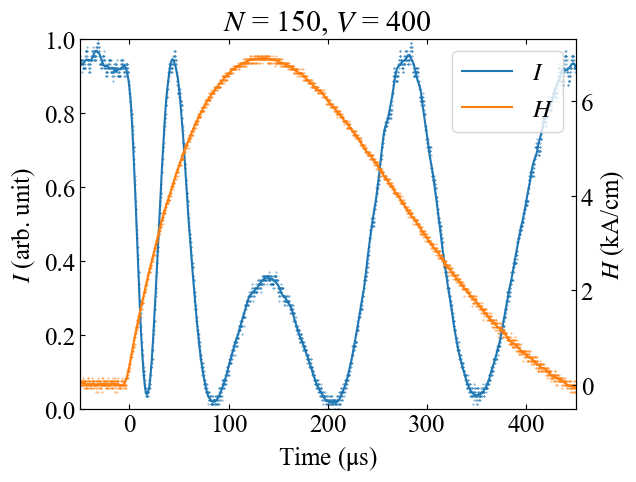
\includegraphics[width = \columnwidth]{xt/01.png}
    \end{minipage}
    \hfill
    \begin{minipage}[t]{0.24\columnwidth}
        \centering
        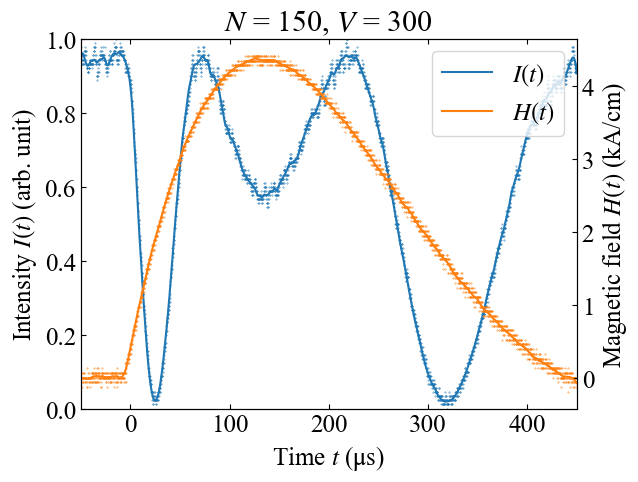
\includegraphics[width = \columnwidth]{xt/02.png}
    \end{minipage}
    \hfill
    \begin{minipage}[t]{0.24\columnwidth}
        \centering
        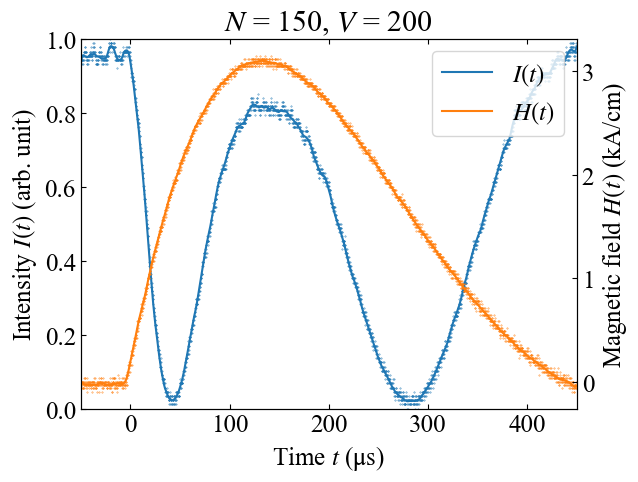
\includegraphics[width = \columnwidth]{xt/03.png}
    \end{minipage}
    \hfill
    \begin{minipage}[t]{0.24\columnwidth}
        \centering
        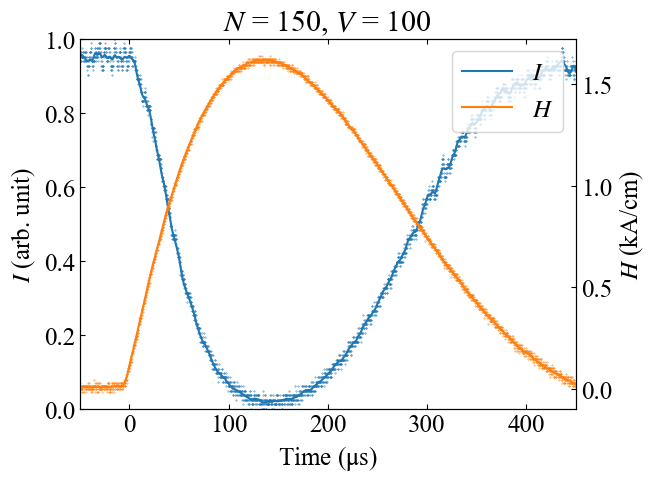
\includegraphics[width = \columnwidth]{xt/04.png}
    \end{minipage}
\end{figure}
\begin{figure}[H]
    \centering
    \begin{minipage}[t]{0.24\columnwidth}
        \centering
        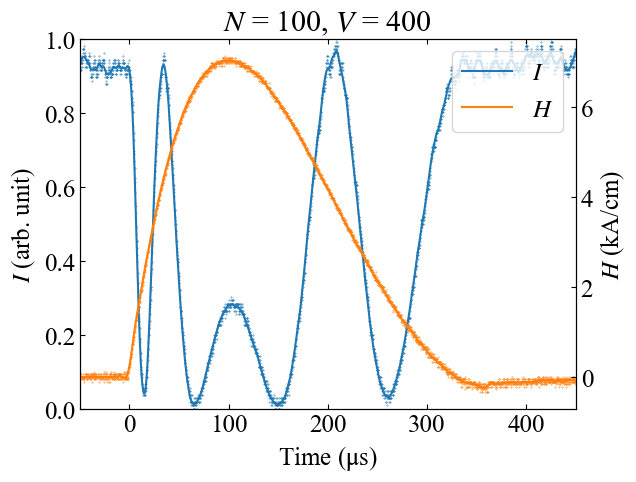
\includegraphics[width = \columnwidth]{xt/05.png}
    \end{minipage}
    \hfill
    \begin{minipage}[t]{0.24\columnwidth}
        \centering
        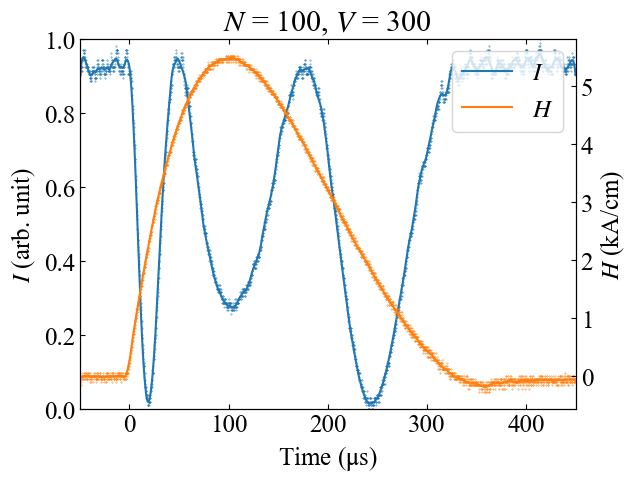
\includegraphics[width = \columnwidth]{xt/06.png}
    \end{minipage}
    \hfill
    \begin{minipage}[t]{0.24\columnwidth}
        \centering
        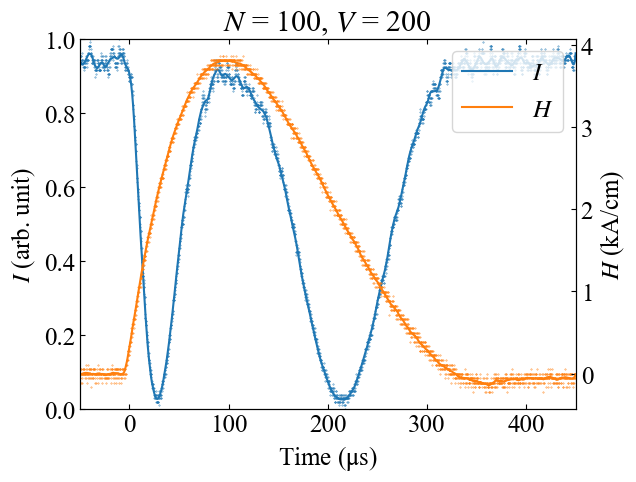
\includegraphics[width = \columnwidth]{xt/07.png}
    \end{minipage}
    \hfill
    \begin{minipage}[t]{0.24\columnwidth}
        \centering
        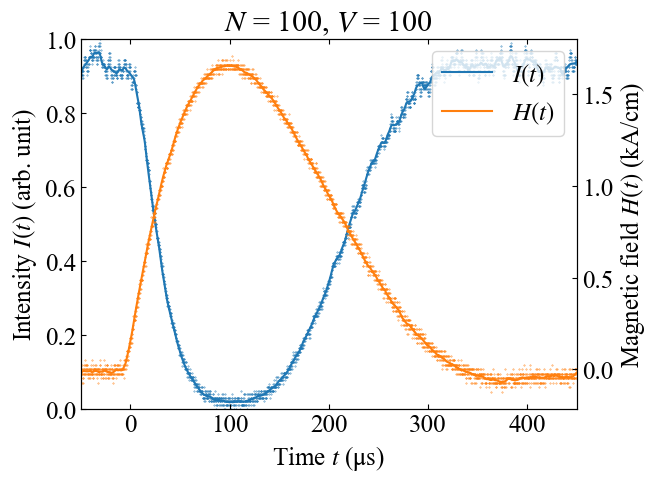
\includegraphics[width = \columnwidth]{xt/08.png}
    \end{minipage}
\end{figure}
\begin{figure}[H]
    \centering
    \begin{minipage}[t]{0.24\columnwidth}
        \centering
        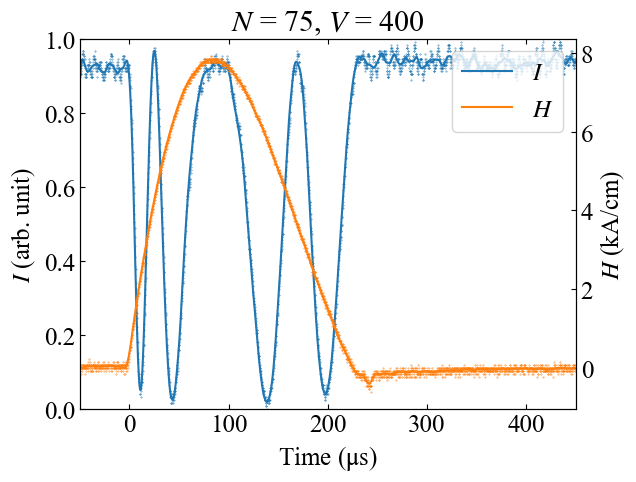
\includegraphics[width = \columnwidth]{xt/09.png}
    \end{minipage}
    \hfill
    \begin{minipage}[t]{0.24\columnwidth}
        \centering
        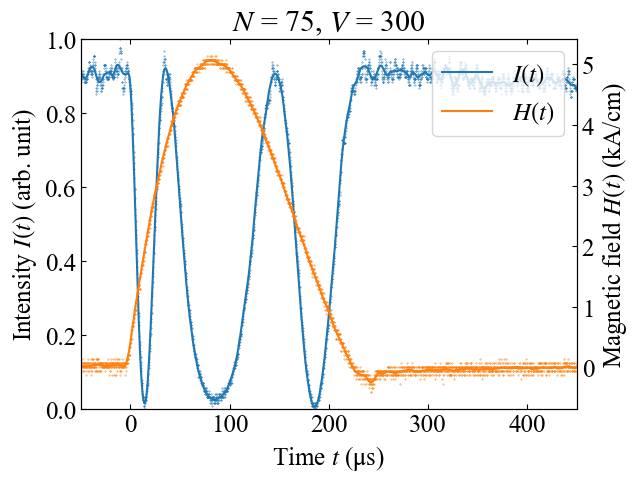
\includegraphics[width = \columnwidth]{xt/10.png}
    \end{minipage}
    \hfill
    \begin{minipage}[t]{0.24\columnwidth}
        \centering
        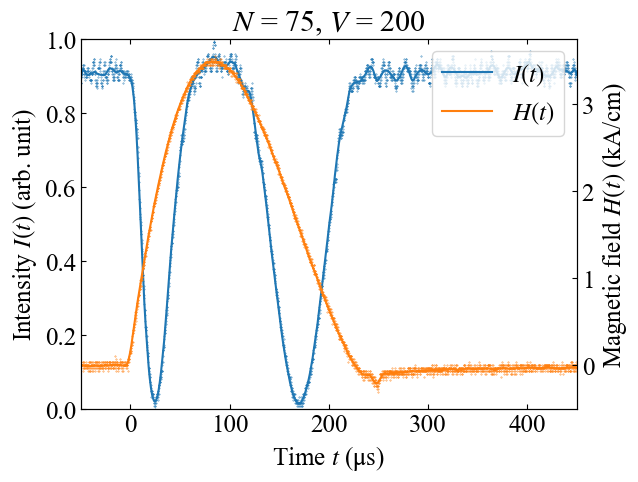
\includegraphics[width = \columnwidth]{xt/11.png}
    \end{minipage}
    \hfill
    \begin{minipage}[t]{0.24\columnwidth}
        \centering
        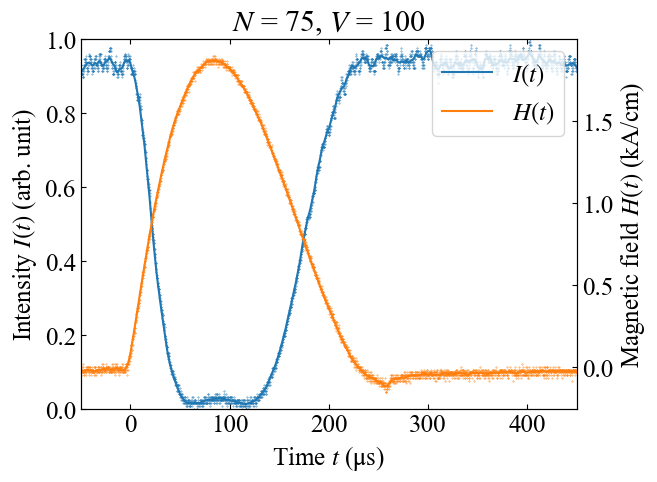
\includegraphics[width = \columnwidth]{xt/12.png}
    \end{minipage}
\end{figure}
\begin{figure}[H]
    \centering
    \begin{minipage}[t]{0.24\columnwidth}
        \centering
        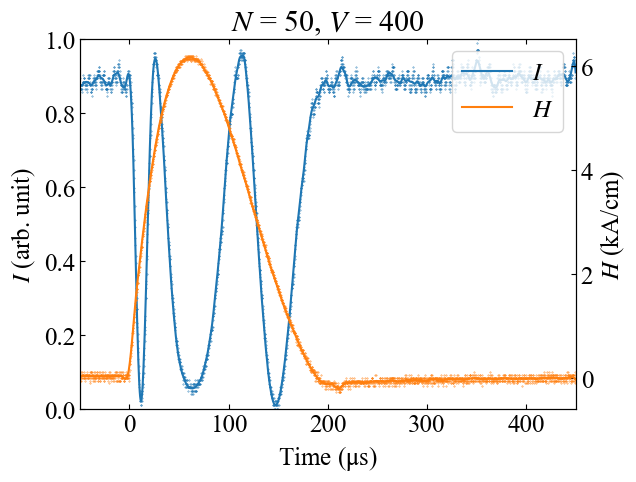
\includegraphics[width = \columnwidth]{xt/13.png}
    \end{minipage}
    \hfill
    \begin{minipage}[t]{0.24\columnwidth}
        \centering
        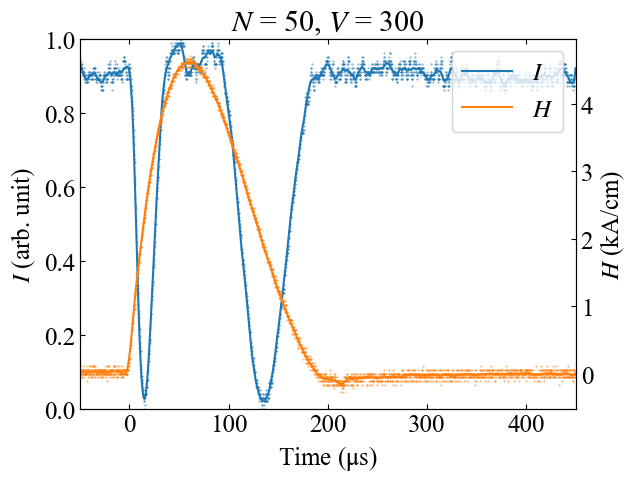
\includegraphics[width = \columnwidth]{xt/14.png}
    \end{minipage}
    \hfill
    \begin{minipage}[t]{0.24\columnwidth}
        \centering
        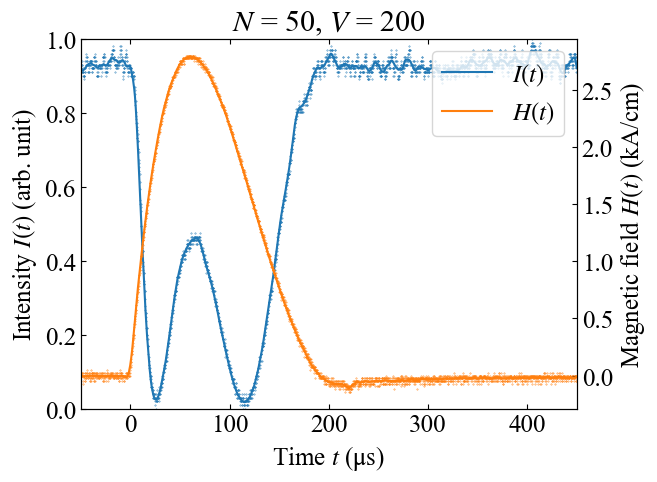
\includegraphics[width = \columnwidth]{xt/15.png}
    \end{minipage}
    \hfill
    \begin{minipage}[t]{0.24\columnwidth}
        \centering
        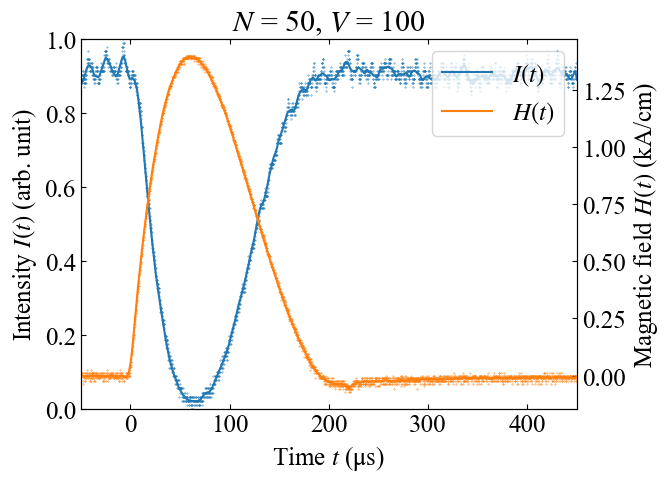
\includegraphics[width = \columnwidth]{xt/16.png}
    \end{minipage}
\end{figure}

次に偏光子と検光子のなす角度が 45 度のときの結果を示す。
\begin{figure}[H]
    \centering
    \begin{minipage}[t]{0.24\columnwidth}
        \centering
        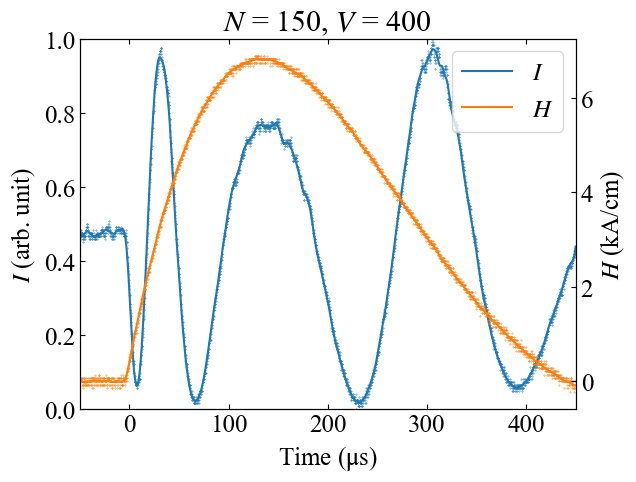
\includegraphics[width = \columnwidth]{xt/17.png}
    \end{minipage}
    \hfill
    \begin{minipage}[t]{0.24\columnwidth}
        \centering
        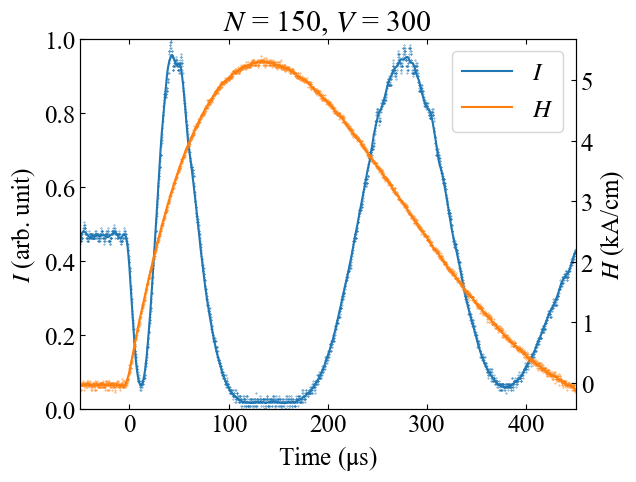
\includegraphics[width = \columnwidth]{xt/18.png}
    \end{minipage}
    \hfill
    \begin{minipage}[t]{0.24\columnwidth}
        \centering
        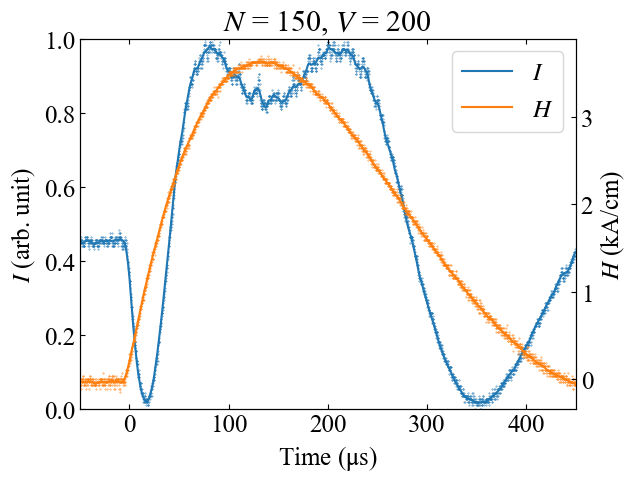
\includegraphics[width = \columnwidth]{xt/19.png}
    \end{minipage}
    \hfill
    \begin{minipage}[t]{0.24\columnwidth}
        \centering
        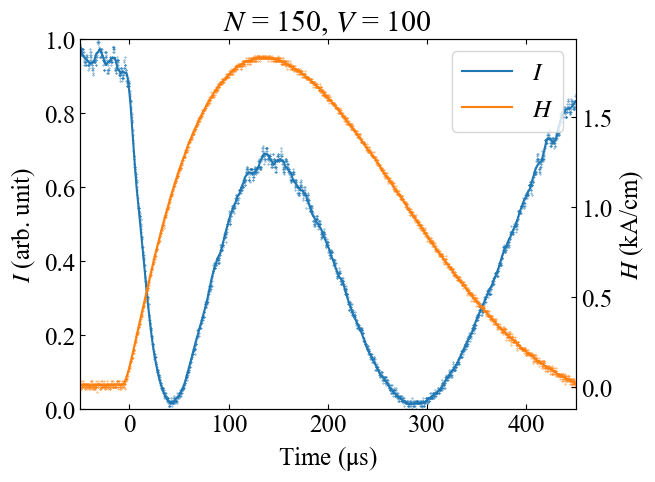
\includegraphics[width = \columnwidth]{xt/20.png}
    \end{minipage}
\end{figure}

最後に磁場の向きを今までの向きとは反平行にして、偏光子と検光子のなす角度が 45 度のときの結果を示す。
\begin{figure}[H]
    \centering
    \begin{minipage}[t]{0.24\columnwidth}
        \centering
        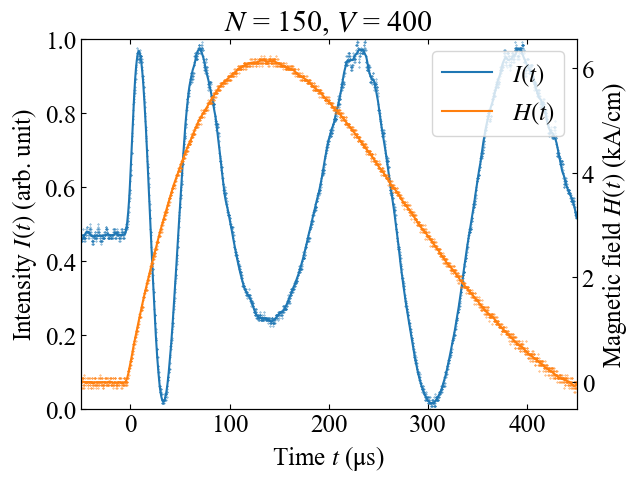
\includegraphics[width = \columnwidth]{xt/22.png}
    \end{minipage}
    \hfill
    \begin{minipage}[t]{0.24\columnwidth}
        \centering
        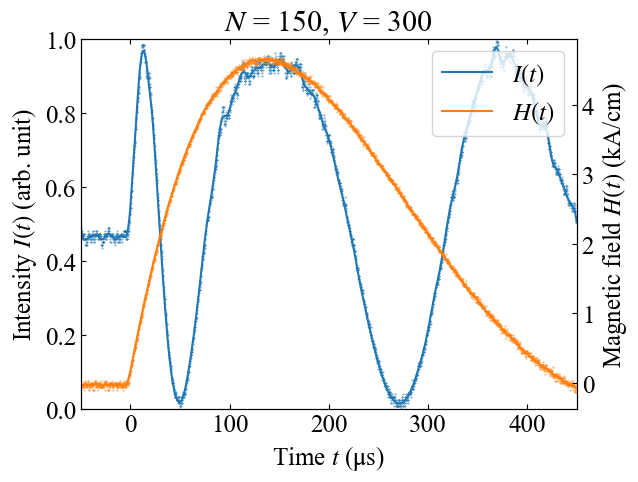
\includegraphics[width = \columnwidth]{xt/23.png}
    \end{minipage}
    \hfill
    \begin{minipage}[t]{0.24\columnwidth}
        \centering
        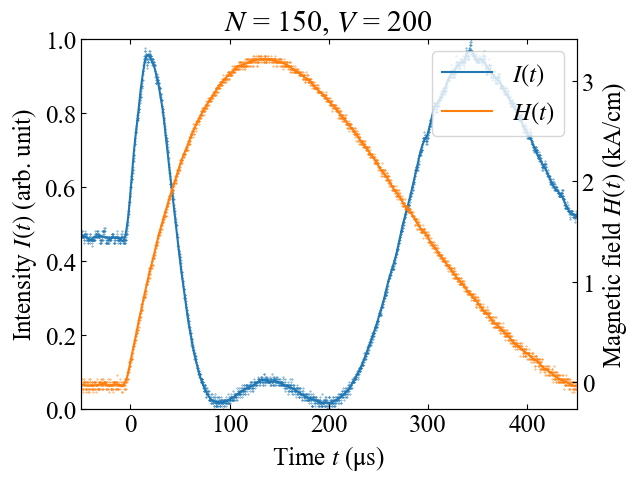
\includegraphics[width = \columnwidth]{xt/24.png}
    \end{minipage}
    \hfill
    \begin{minipage}[t]{0.24\columnwidth}
        \centering
        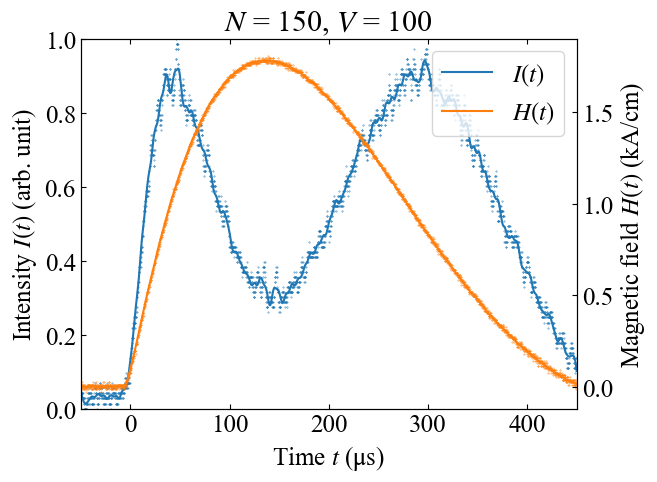
\includegraphics[width = \columnwidth]{xt/25.png}
    \end{minipage}
\end{figure}

\subsection{x-y グラフ}

横軸に磁場の強さ (kA/cm)、縦軸に透過光の強度 (arb. unit) をプロットしたグラフは以下の通りである。
磁場による磁気ガラス中の磁化の応答が遅れるがあるため、
それを補正したものと補正していないもの両方を載せる。

補正はこのようにして行った。
磁場の強さと透過光の強度の x-y グラフを作る際に、
時刻\(t[i]\)のときの磁場の強さと透過光を\(H[i], I[i]\)というようにおく。
磁化の応答が遅れるということは、同じだけ透過光の応答も遅らせればよい。
なので
\begin{align}
    (H[i], I[i+\text{shift}])
\end{align}
というように光強度も shift の分だけ遅らせたペアの点をプロットするというようにして補正した。

グラフの上部にあるのはソレノイドコイルの巻き数とパルス発生装置の充電電圧、どれだけシフトしたかの量である。

始めに偏光子と検光子のなす角度が 0 度のときの結果を示す。
\begin{figure}[H]
    \centering
    \begin{minipage}[t]{0.24\columnwidth}
        \centering
        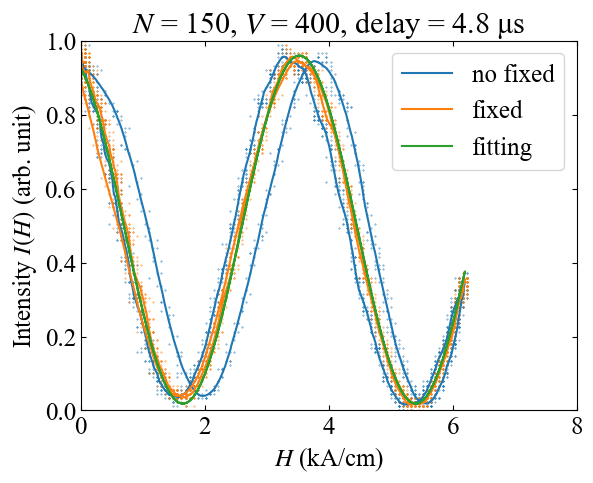
\includegraphics[width = \columnwidth]{xy/01.png}
    \end{minipage}
    \hfill
    \begin{minipage}[t]{0.24\columnwidth}
        \centering
        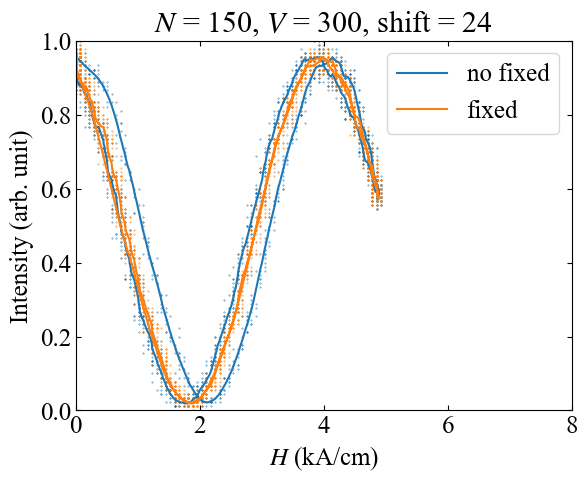
\includegraphics[width = \columnwidth]{xy/02.png}
    \end{minipage}
    \hfill
    \begin{minipage}[t]{0.24\columnwidth}
        \centering
        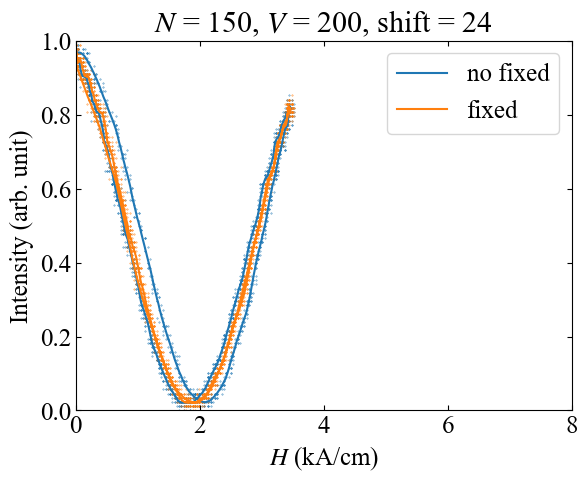
\includegraphics[width = \columnwidth]{xy/03.png}
    \end{minipage}
    \hfill
    \begin{minipage}[t]{0.24\columnwidth}
        \centering
        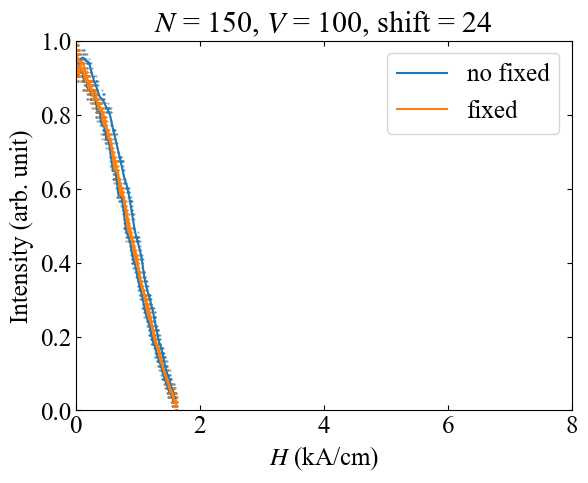
\includegraphics[width = \columnwidth]{xy/04.png}
    \end{minipage}
\end{figure}
\begin{figure}[H]
    \centering
    \begin{minipage}[t]{0.24\columnwidth}
        \centering
        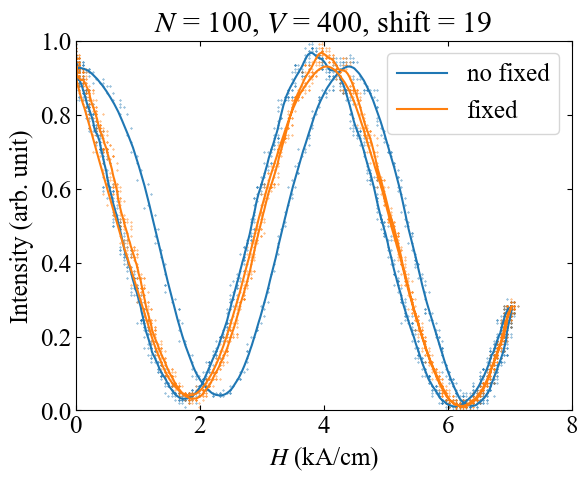
\includegraphics[width = \columnwidth]{xy/05.png}
    \end{minipage}
    \hfill
    \begin{minipage}[t]{0.24\columnwidth}
        \centering
        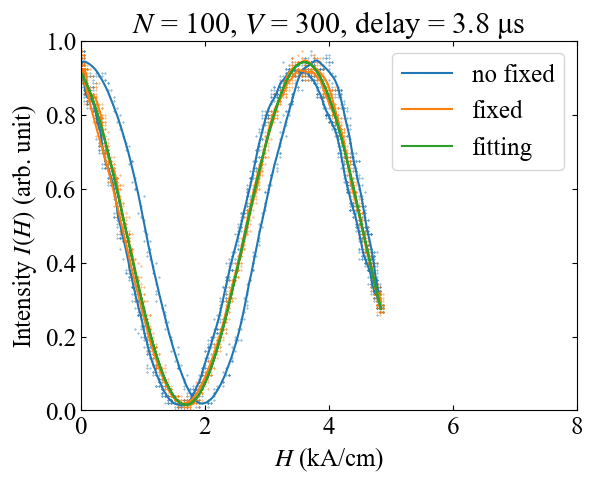
\includegraphics[width = \columnwidth]{xy/06.png}
    \end{minipage}
    \hfill
    \begin{minipage}[t]{0.24\columnwidth}
        \centering
        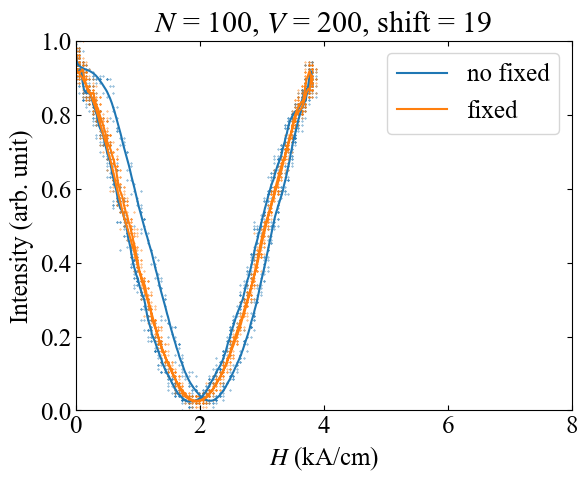
\includegraphics[width = \columnwidth]{xy/07.png}
    \end{minipage}
    \hfill
    \begin{minipage}[t]{0.24\columnwidth}
        \centering
        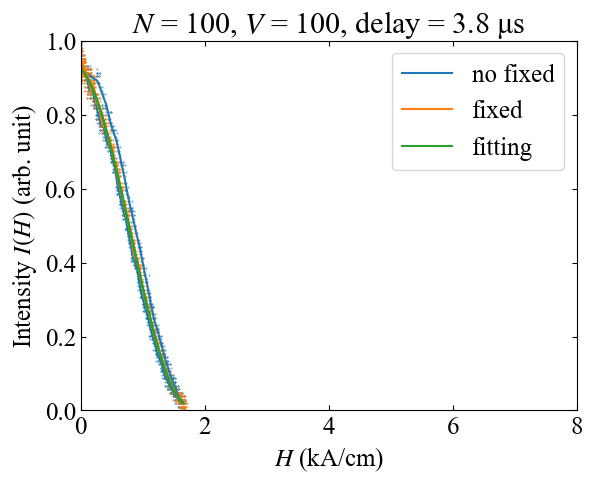
\includegraphics[width = \columnwidth]{xy/08.png}
    \end{minipage}
\end{figure}
\begin{figure}[H]
    \centering
    \begin{minipage}[t]{0.24\columnwidth}
        \centering
        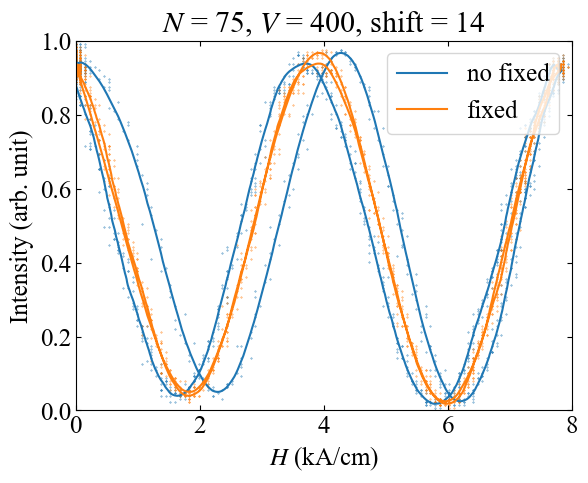
\includegraphics[width = \columnwidth]{xy/09.png}
    \end{minipage}
    \hfill
    \begin{minipage}[t]{0.24\columnwidth}
        \centering
        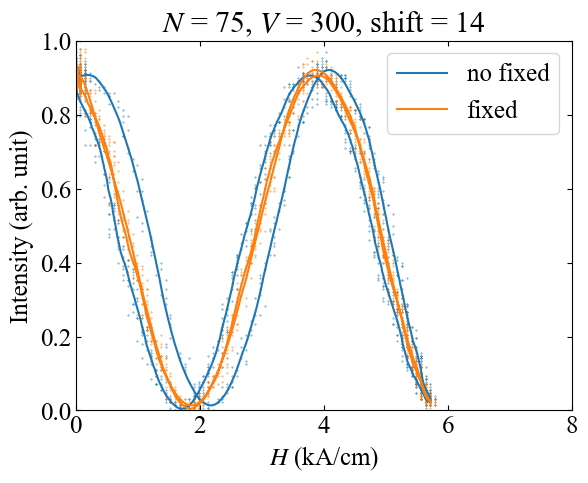
\includegraphics[width = \columnwidth]{xy/10.png}
    \end{minipage}
    \hfill
    \begin{minipage}[t]{0.24\columnwidth}
        \centering
        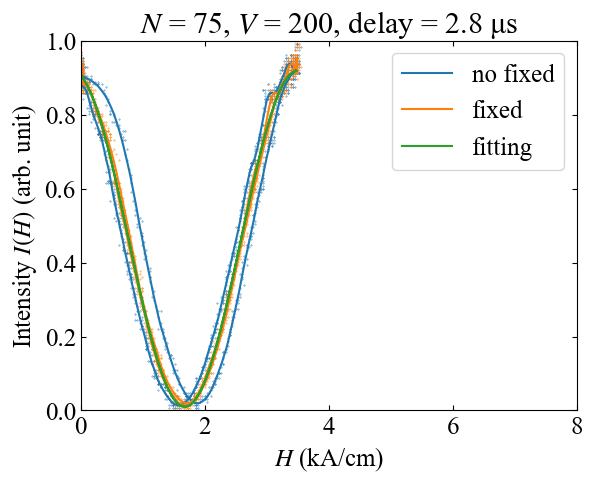
\includegraphics[width = \columnwidth]{xy/11.png}
    \end{minipage}
    \hfill
    \begin{minipage}[t]{0.24\columnwidth}
        \centering
        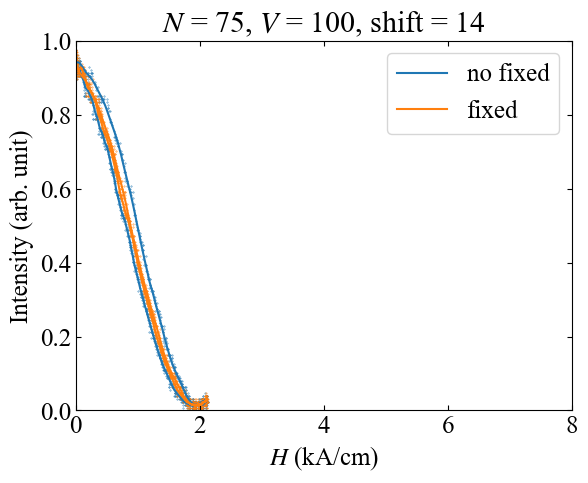
\includegraphics[width = \columnwidth]{xy/12.png}
    \end{minipage}
\end{figure}
\begin{figure}[H]
    \centering
    \begin{minipage}[t]{0.24\columnwidth}
        \centering
        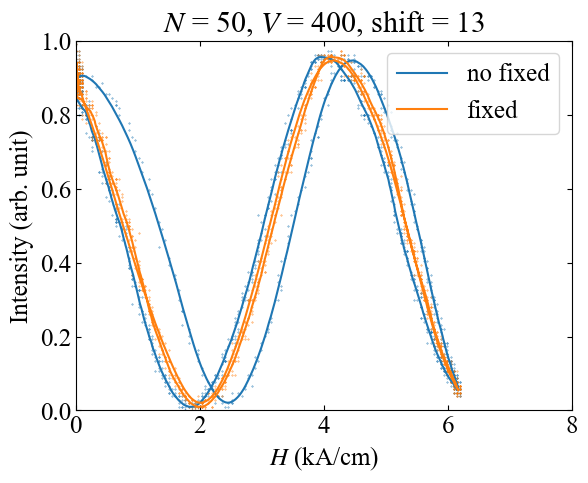
\includegraphics[width = \columnwidth]{xy/13.png}
    \end{minipage}
    \hfill
    \begin{minipage}[t]{0.24\columnwidth}
        \centering
        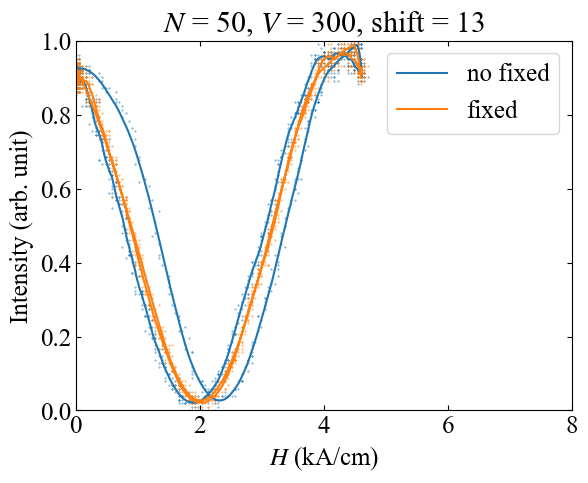
\includegraphics[width = \columnwidth]{xy/14.png}
    \end{minipage}
    \hfill
    \begin{minipage}[t]{0.24\columnwidth}
        \centering
        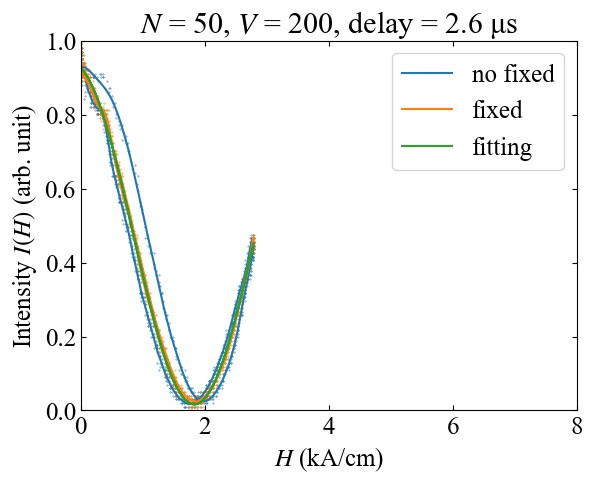
\includegraphics[width = \columnwidth]{xy/15.png}
    \end{minipage}
    \hfill
    \begin{minipage}[t]{0.24\columnwidth}
        \centering
        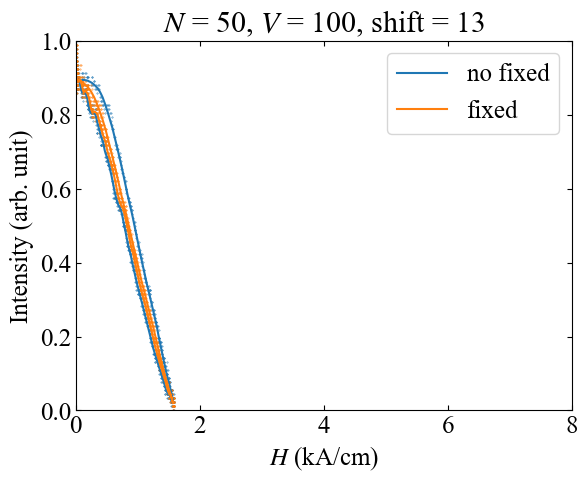
\includegraphics[width = \columnwidth]{xy/16.png}
    \end{minipage}
\end{figure}

次に偏光子と検光子のなす角度が 45 度のときの結果を示す。
\begin{figure}[H]
    \centering
    \begin{minipage}[t]{0.24\columnwidth}
        \centering
        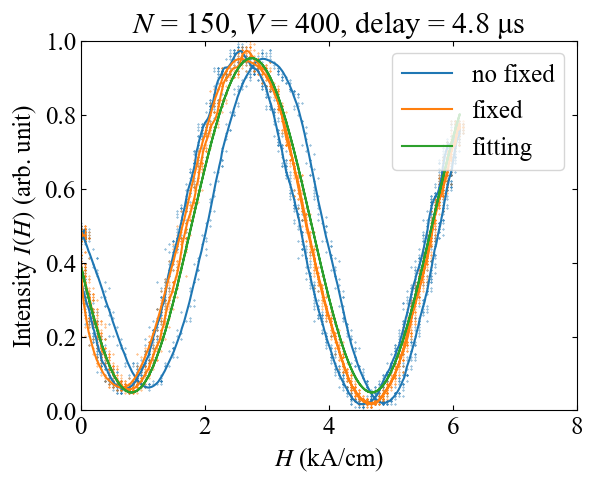
\includegraphics[width = \columnwidth]{xy/17.png}
    \end{minipage}
    \hfill
    \begin{minipage}[t]{0.24\columnwidth}
        \centering
        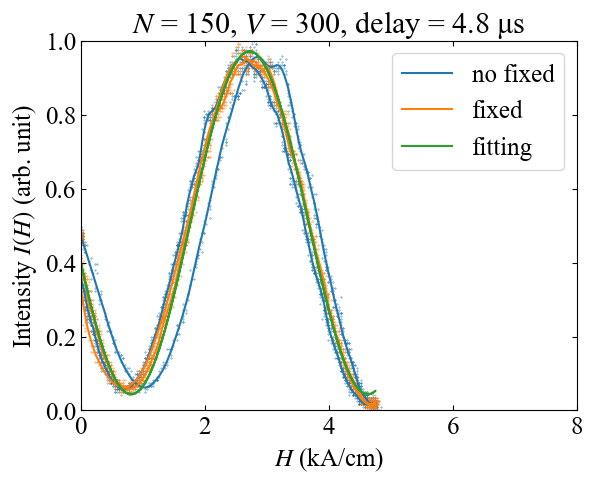
\includegraphics[width = \columnwidth]{xy/18.png}
    \end{minipage}
    \hfill
    \begin{minipage}[t]{0.24\columnwidth}
        \centering
        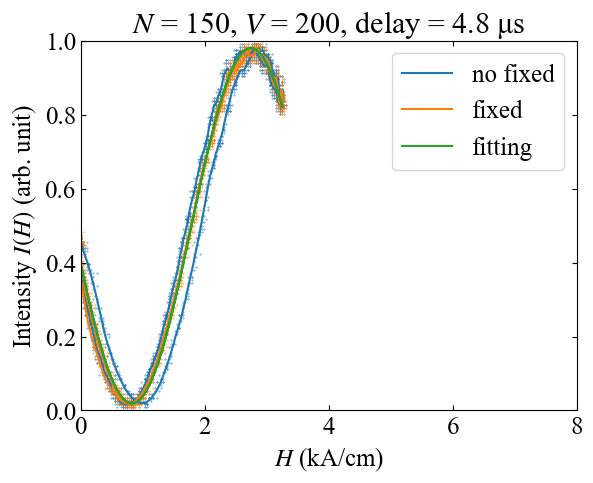
\includegraphics[width = \columnwidth]{xy/19.png}
    \end{minipage}
    \hfill
    \begin{minipage}[t]{0.24\columnwidth}
        \centering
        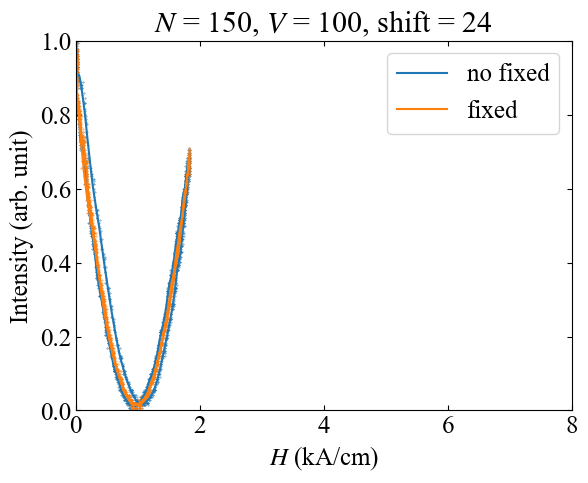
\includegraphics[width = \columnwidth]{xy/20.png}
    \end{minipage}
\end{figure}

最後に磁場の向きを今までの向きとは反平行にして、偏光子と検光子のなす角度が 45 度のときの結果を示す。
\begin{figure}[H]
    \centering
    \begin{minipage}[t]{0.24\columnwidth}
        \centering
        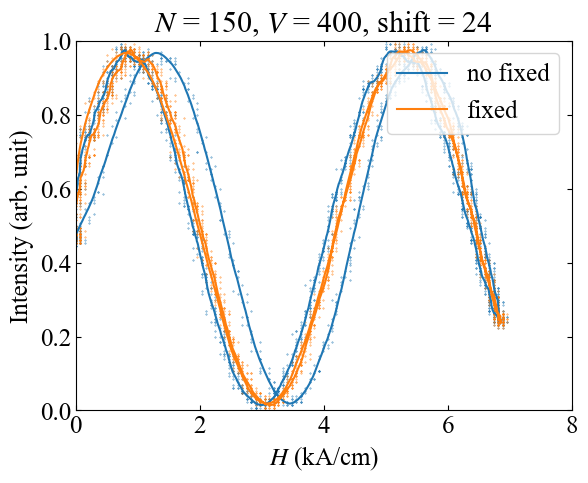
\includegraphics[width = \columnwidth]{xy/22.png}
    \end{minipage}
    \hfill
    \begin{minipage}[t]{0.24\columnwidth}
        \centering
        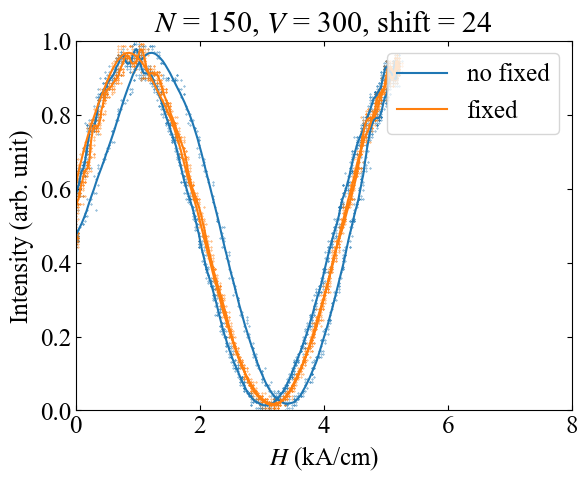
\includegraphics[width = \columnwidth]{xy/23.png}
    \end{minipage}
    \hfill
    \begin{minipage}[t]{0.24\columnwidth}
        \centering
        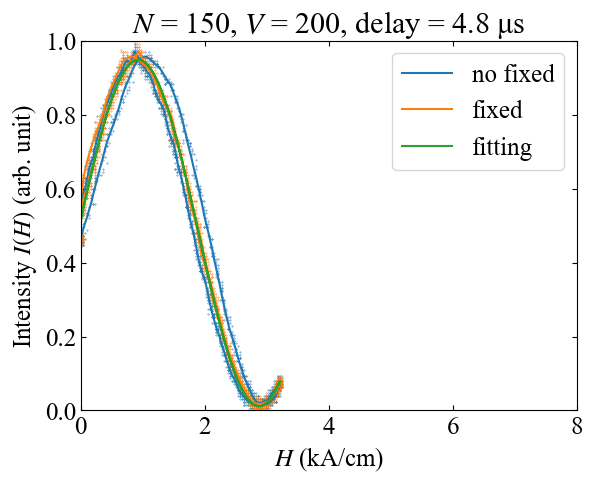
\includegraphics[width = \columnwidth]{xy/24.png}
    \end{minipage}
    \hfill
    \begin{minipage}[t]{0.24\columnwidth}
        \centering
        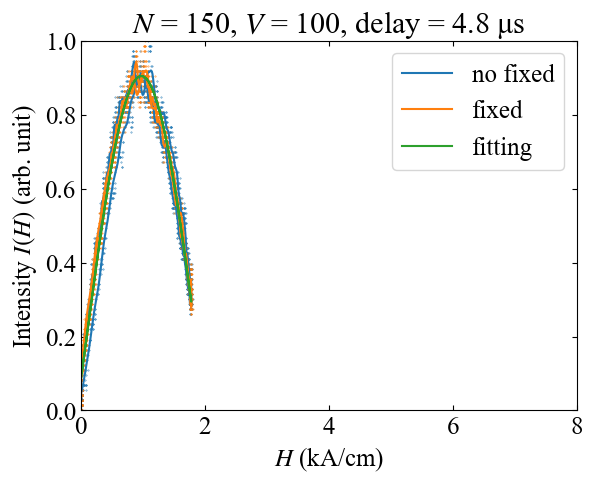
\includegraphics[width = \columnwidth]{xy/25.png}
    \end{minipage}
\end{figure}
\fi

\end{document}